\chapter{Learning Words Like Humans Do: Syntactic Smoothing for Language Model Training}

While the previous chapter explored curriculum learning as a way to structure the input space and learning trajectory of a model, we now turn to a complementary question: \emph{how can internal representations themselves be shaped to better support generalization—particularly for low-frequency vocabulary?} Just as children benefit from structured exposure to language, they also rely heavily on syntactic cues to make sense of unfamiliar words. This chapter investigates how language models might likewise leverage structural signals to improve lexical generalization.

One of the most striking capabilities of human learners is their ability to infer the meaning of unknown words from syntactic and semantic context. Consider the sentence: ``the Golden Gate Bridge has been \emph{obnebulated} every morning this week, limiting visibility of the Pacific Ocean.'' Although most readers will not have encountered the word \textit{obnebulated}, we can make two confident inferences: (1) it is a verb, likely in the past participle form (given the ``has been'' auxiliary and the \textit{-ed} suffix), and (2) its meaning relates to fog or visibility. Human learners use this type of syntactic bootstrapping constantly—inferring semantic properties from grammatical structure long before they've memorized a full lexicon.

\begin{figure}[ht!]
    \centering
    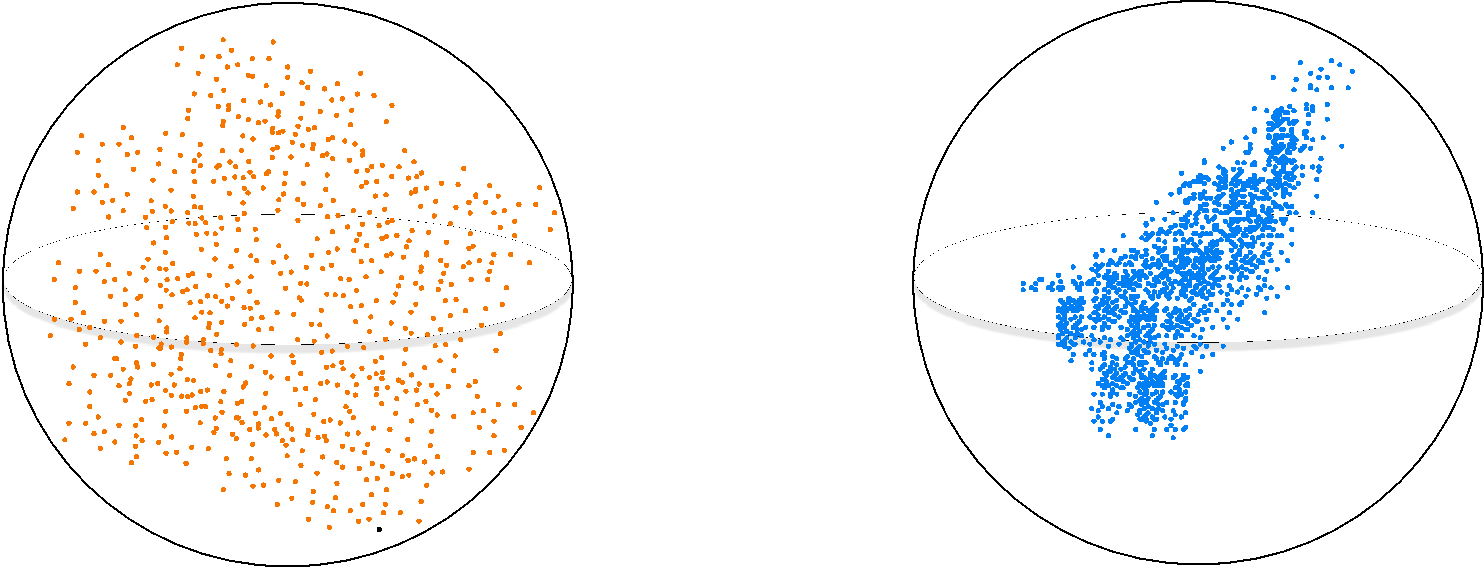
\includegraphics[width=0.8\linewidth]{chapters/syntatic-smoothing/figures/anisotropy_visualization.pdf}
    \caption{Artistic visualization of the representational space of a language model, showing the clustering of tokens into a narrow manifold. The model is trained with a maximum likelihood objective, and the representations of the tokens are clustered together into a narrow manifold.}
    \label{fig:anisotropy_visualization}
\end{figure}

This ability is notably lacking in current language models. Despite their success on many NLP benchmarks \citep{touvron2023llama, chowdhery2023palm}, pre-trained transformer language models (PLMs) still struggle with rare or unseen words. A key reason is thattvast majority of language models are pre-trained to maximize the log-likelihood of a word, given the surrounding context \citep{devlin2019bert, brown2020gpt3, chowdhery2023palm, touvron2023llama}. As language use is characterized by a Zipfian distribution \citep{zipf1935zipflaw}, language models are exposed to frequent tokens exponentially more often than infrequent ones during pre-training. Consequently, the representations of these frequent tokens are optimized based on exponentially more learning signals than those of low-frequency tokens. It has been shown that maximum likelihood objectives lead to representation degeneration in English language models because infrequent tokens are pushed into a narrow manifold of the representational space \citep{gao2018representation}. This representation degeneration problem is linked to the broader problem of \textbf{anisotropy}: the hidden states of a language model tend to cluster together into a small cone-shaped subspace, rather than over their full representational capacity \citep{arora2016latent, ethayarajh2019contextual, gao2018representation}. \cref{fig:anisotropy_visualization} illustrates this phenomenon. As language model evaluation is based on cumulative evaluation scores that conceal how well a model processes infrequent words, the disparities in the representational space are difficult to assess. 

Our work makes two key contributions:

First, this chapter introduces \textbf{\texttt{Syntactic Smoothing}}, a simple but cognitively motivated method for improving the representation of infrequent tokens during language model training. Inspired by the human tendency to group unknown words with structurally similar known words, we propose redistributing part of the learning signal for each token across other tokens that share similar syntactic roles. Using this method, tokens that are seldom seen during training benefit from the more frequent updates of tokens that occur in similar syntactic functions.  In effect, infrequent tokens benefit from updates to their syntactic neighbors—allowing them to ``learn by association,'' as children often do.

Next, we quantify the impact of this approach using a new diagnostic measure of \textbf{frequency bias}—a model's tendency to prefer grammatical sentences that contain high-frequency tokens over those with low-frequency ones. We show that \texttt{Syntactic Smoothing} reduces both frequency bias and anisotropy, and does so without hurting performance on downstream tasks. These findings suggest that small structural changes to the learning process—rooted in cognitive observations—can meaningfully improve the robustness and interpretability of language models.

The remainder of this chapter is organized as follows: Section~\ref{sec:related-literature} reviews the related literature on frequency bias and anisotropy in language models. Section~\ref{sec:smoothing-method} introduces the \texttt{Syntactic Smoothing} method and details its implementation. Section~\ref{subsection:experimental_setup} describes the experimental setup and implementation of \texttt{Syntactic Smoothing}. Section~\ref{sec:results} both presents our results and analysis across synthetic and real-world evaluations and discusses the implications of our findings. Finally, Section~\ref{sec:conclusion} summarizes our work and motivates further exploration of how language models internalize linguistic structure over time.

\section{Related Literature}
\label{sec:related-literature}

Through maximum likelihood training, language models implicitly learn to encode token frequency statistics. This training process gives rise to a frequency bias in models that constrains their ability to generalize to infrequent tokens. In this section, we begin by reviewing literature that discusses the challenges of generalizing linguistic knowledge to infrequent tokens. We then examine recent work that links the impact of token frequency to anisotropy in the models' representational space.

\subsection{Generalization to Infrequent Tokens}

Current approaches to language modeling rely heavily on the memorization of infrequent tokens to perform well on downstream tasks \citep{feldman2020does}. Recent analytical work has shown that certain layers of transformer models implicitly store memorized long-tail data \citep{haviv2023understanding, kobayashi2023transformer}. \citet{feldman2020neural} demonstrate that models memorize atypical examples to achieve the highest accuracy on long-tailed data samples. This memorization hack, however, has only been shown to work well with over-parameterized models \citep{belkin2019reconciling}. While these studies present various metrics to evaluate memorization, these metrics do not capture how memorization impacts generalized linguistic understanding within the models. In our work, we address this gap by developing a metric that quantifies the extent of this frequency bias in relation to models' linguistic abilities.

Language use follows a Zipfian distribution, meaning that many tokens appear infrequently. Standard training objectives often require large models and noisy datasets with sufficient long-tail samples for effective generalization \citep{zheng2022memorization}. However, improving generalization without excessive scaling can be achieved by training models with inductive priors that leverage linguistic information. On the lexical level, the integration of morphological and orthographic information during representation learning has been explored to obtain more fine-grained word embeddings \citep{salle2018incorporating, vulic2017morphfitting, cotterel2015morphological, bhatia2016morphological, botha2014compositional}. To improve syntactic generalization, the objective function has been enriched with auxiliary tasks, such as predicting constituency labels \citep{wang2023language}, hypernyms \citep{bai2022better}, dependency tags \citep{cui2022lert}, and POS tags \citep{diehlmartinez2023climb}. Some approaches have also shown promising results on rare word performance by constructing token embeddings that consider a word's surface form and surrounding context \citep{schick2019attentive, schick2020rare}.

\subsection{Anisotropy in Representational Space}
While frequency bias and generalization capabilities can be observed by analyzing model behavior on input--output patterns, representational analyses indicate that these phenomena are linked to the distribution of token representations. Language models trained as likelihood maximizers have been shown to yield degenerate representations for rare tokens \citep{gao2018representation}. Throughout training, infrequent tokens are disproportionately pushed in the negative direction of most hidden states, resulting in their clustering together irrespective of their semantic or syntactic properties. This clustering behavior leads to anisotropy: rather than occupying a large region of the representational space, token representations lie along a narrow manifold \citep{gao2018representation, ethayarajh2019contextual}

\subsubsection{Defining Anisotropy}

Anisotropy is defined as the inverse of isotropy: $1-I(v(\cdot))$. A representational space is isotropic if all the vector directions are distributed uniformly, meaning no particular direction is favored over another.

\citeauthor{arora2016latent}\ and \citeauthor{mu2018all} define isotropy as:

\begin{equation}
    I(v(\cdot)) \coloneq \frac{\min_{\norm{c}=1} Z(c)}{\max_{\norm{c}=1} Z(c)}
\end{equation}
where $c$ is a unit vector and $Z(c)$ is defined as the partition function over all tokens $w$ in the vocabulary $V$ , with representations $v(w)$:
$$
    Z(c) = \sum_{w \in V} \exp(c^Tv(w))
$$
In practice, this definition of isotropy is analytically infeasible to solve. In this paper, we follow an empirical approximation proposed by \citeauthor{ethayarajh2019contextual}: 
\begin{equation}
\label{eq:empirical-isotropy}
    I(v(\cdot)) \coloneq \mathbb{E}_{i\ne j}\big(1-\cos(v(w_i), v(w_j))\big)
\end{equation}
Here, $w_i$ and $w_j$ are two tokens sampled from the vocabulary, and $\cos$ is defined as taking the cosine similarity of the two word representations for $w_i$ and $w_j$.  

Despite its prevalence, the impact of anisotropy on a model's language understanding abilities remains unclear. Some studies suggest that reducing anisotropy improves performance on non-contextual benchmarks, sentence comparison tasks, and multilingual benchmarks \citep{bis2021too, su2021whitening, rajaee2022isotropy}. Conversely, other research indicates that higher anisotropy might enhance semantic clustering tasks and that reducing anisotropy does not uniformly improve performance on common NLU tasks \citep{ait2023anisotropy, ding2022isotropy}. Furthermore, the relationship between anisotropy and maximum likelihood training has been questioned. Some researchers argue that isotropy exists in local manifolds of contextual word representations \citep{cai2020isotropy}, while others contend that anisotropy arises from the learning dynamics of the query and key attention matrices in transformer models \citep{godey2024anisotropy}.

\subsubsection{Reducing Anisotropy}

Existing methods to reduce anisotropy broadly fall into three categories. The first group of approaches transforms the hidden states of language models to remove semantically uninformative directions and to preserve the dimensions of maximal isotropy \citep{arora2016simple, mu2018all, raunak2019effective, su2021whitening,bis2021too}. This intervention style is based on the assumption that the top singular dimensions of pre-trained word representations encode frequency statistics rather than semantic or lexical information \citep{mu2018all}. The second category of methods introduces novel training objectives and regularization terms that reduce the effects of anisotropy \citep{gong2018frage, gao2018representation, wang2019improving}. This type of approach places an inductive bias on representations that push the embeddings of frequent and infrequent words to occupy a similar semantic space. The third set of approaches explores different training paradigms to directly minimize anisotropy, such as using normalizing flow models \citep{li2020sentence} or manipulating the gradients used in maximum likelihood models \citep{yu2022rare}

\vspace{1em}

While frequency bias and anisotropy are prevalent in language modeling, quantifying their effects and understanding their impact on generalization, particularly for infrequent words, remains an open area of research. Our paper introduces a novel method for improving the representation of infrequent tokens by integrating linguistic information. Moreover, we hypothesize that adjusting the learning process to better represent infrequent tokens will also reduce anisotropy, as these two phenomena are interconnected.

\section{Frequency Bias}
\label{section:freq-bias}

\begin{figure}[ht!]
    \centering
    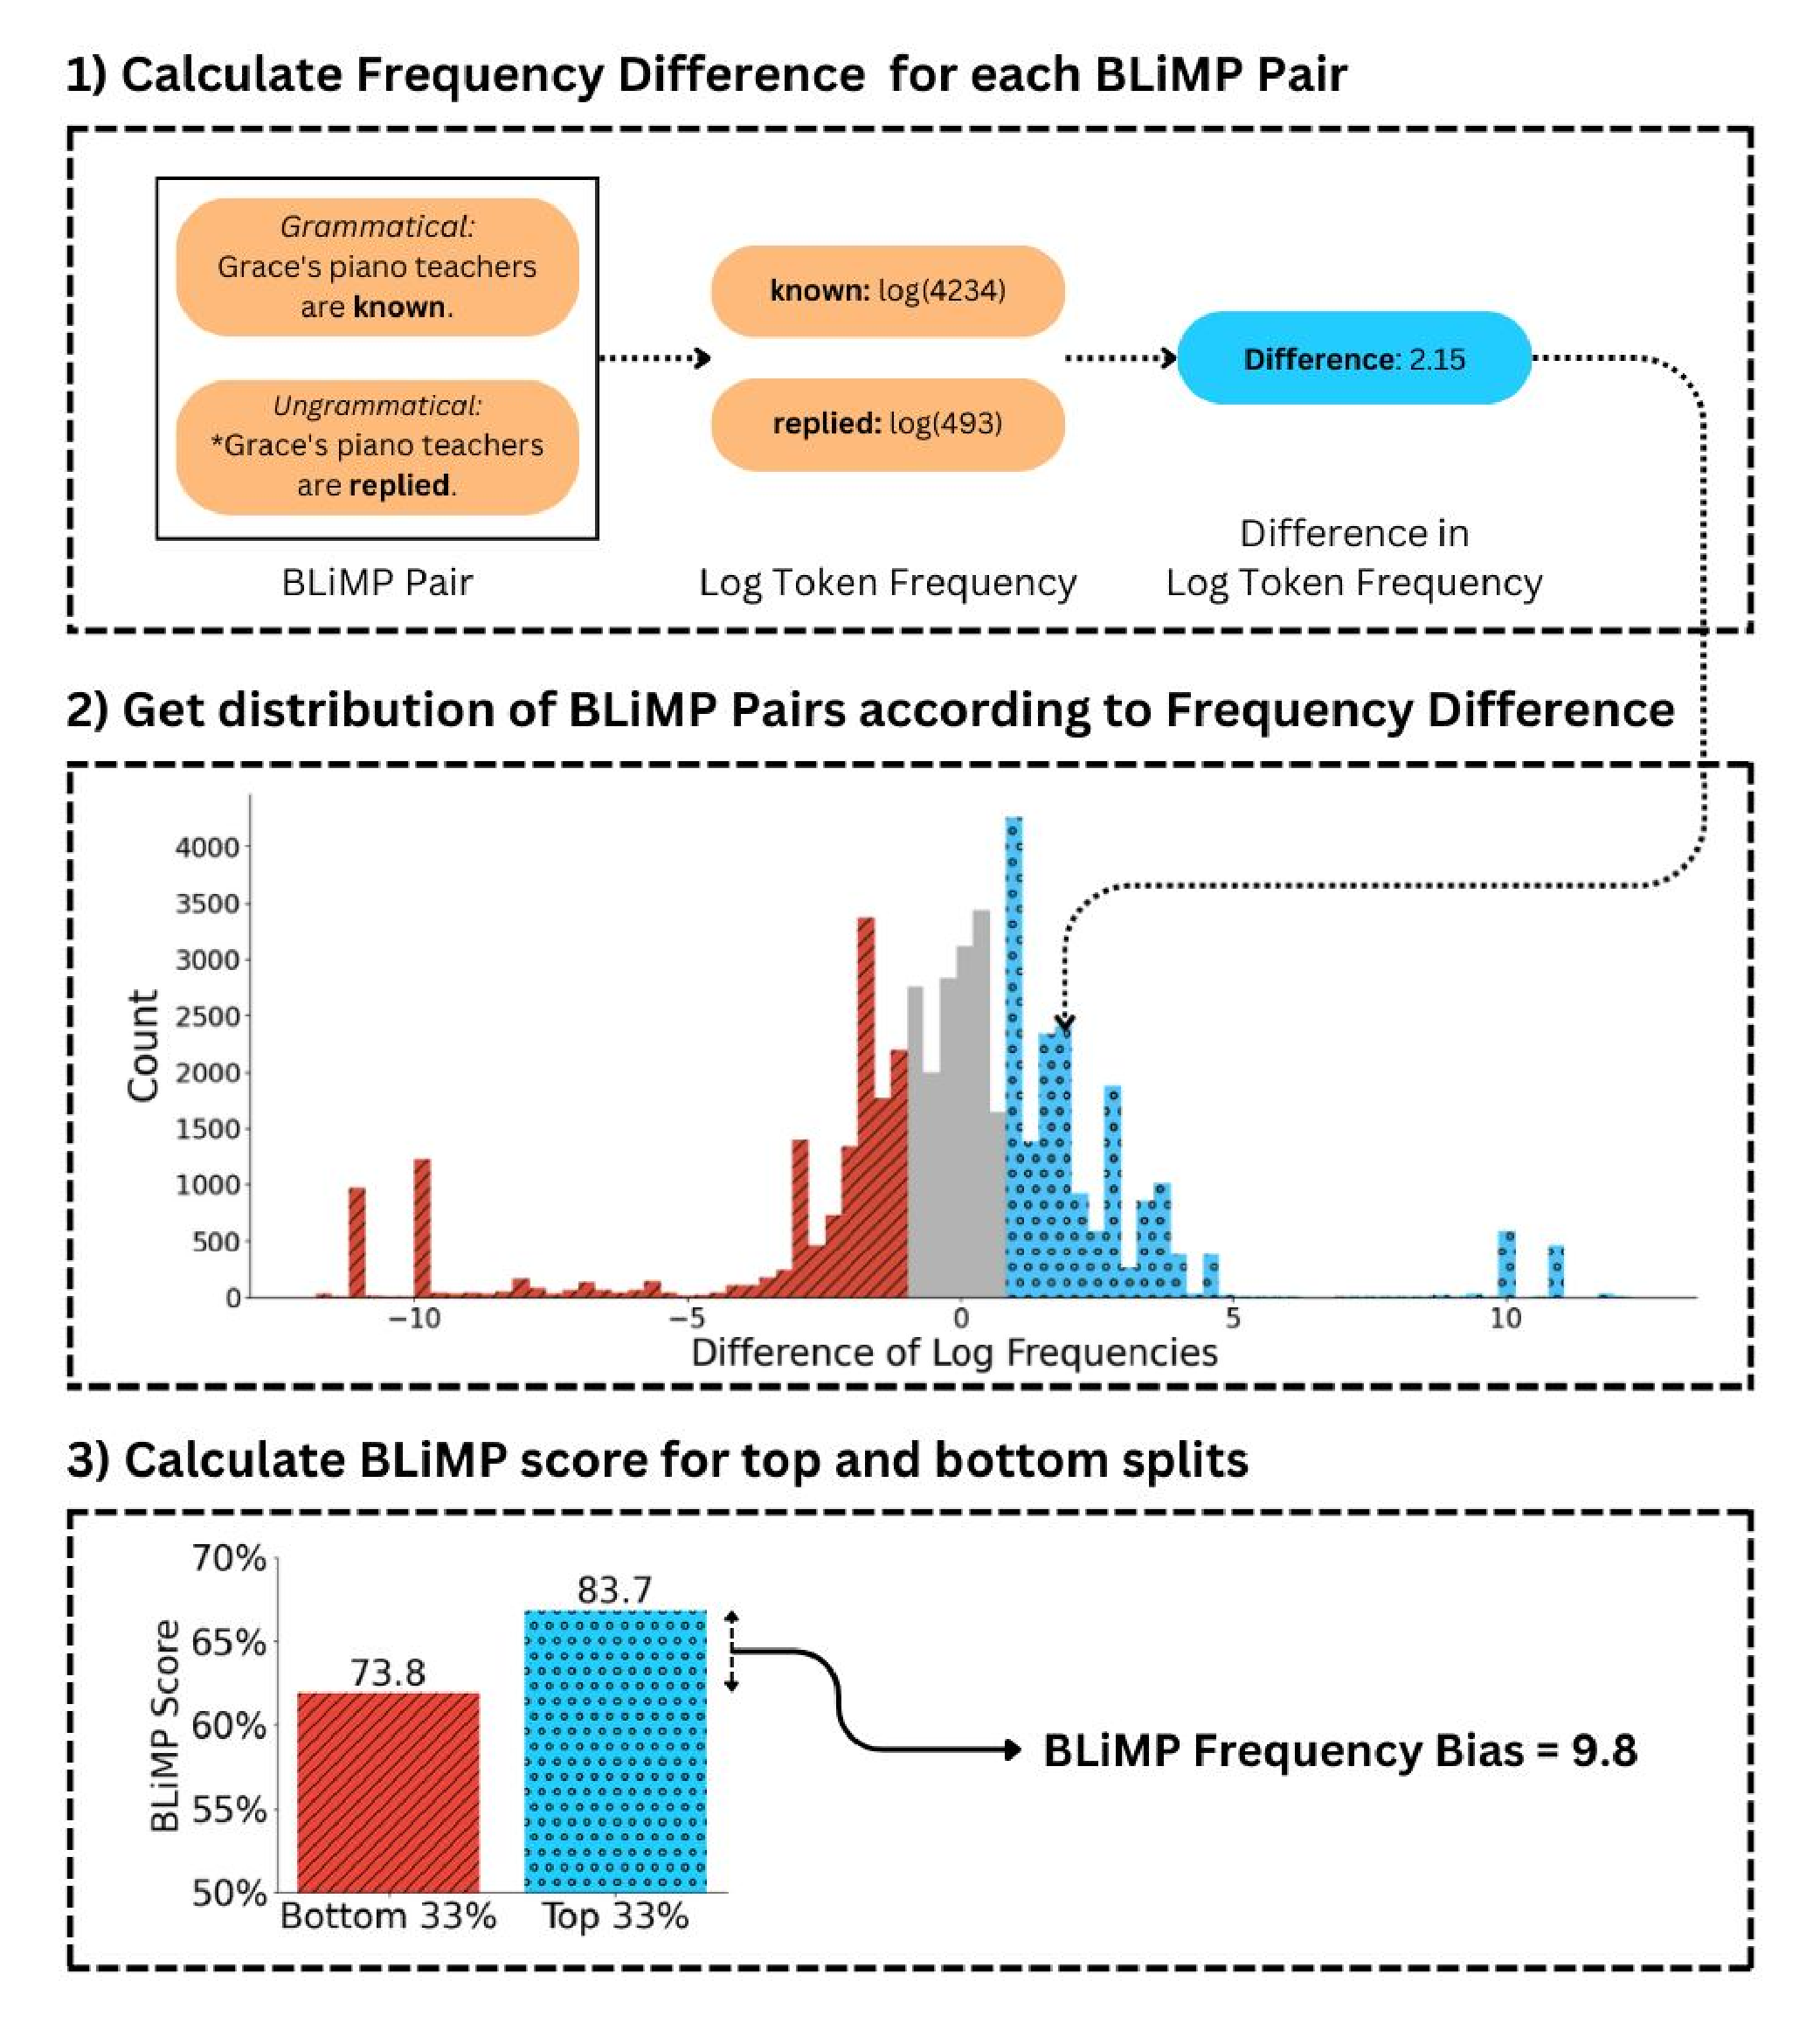
\includegraphics[width=0.8\linewidth]{chapters/syntatic-smoothing/figures/blimp_bias_example.pdf}
    \caption{Illustration of the BLiMP \textbf{frequency bias} calculation used to evaluate a model's reliance on frequency statistics when making predictions. The example BLiMP values are from a baseline RoBERTa model.}
    \label{fig:blimp_bias}
    \vspace{-1em}
\end{figure}

BLiMP is carefully balanced to ensure individual tokens occur equally in both sentence types. However, within a single pair, there may be an imbalance in average token frequency: For instance, the sentence
\textit{Grace's piano teachers are \textbf{known}} has a log frequency of 8.35 while its associated minimal pair \textit{Grace's piano teachers are \textbf{replied}} has a log frequency of 6.20.  We hypothesize that despite the minimal difference in BLiMP pairs, models trained in a typical manner will be biased by token frequency when determining grammatical acceptability.

Our goal is to quantify how language model performance differs between BLIMP pairs with large positive frequency differences (where the correct sentence has more frequently occurring tokens) and with large negative frequency differences (where the correct sentence has much less frequently occurring tokens). We do so in three steps.

First, we minimally preprocess BLiMP to ensure our analysis focuses on meaningful token-level differences. Specifically, we filter the dataset to only include sentence pairs where one set of tokens has been replaced by another set (e.g., "The cat sat" vs "The dog sat"). We exclude sentence pairs that differ only in token order (e.g., "The cat sat" vs "Sat the cat") or where tokens have been added to one sentence but not replaced (e.g., "The cat sat" vs "The cat sat quietly"). This filtering process removes approximately 15\% of the original BLiMP pairs and 9 of the 67 linguistic subtasks from consideration, but ensures that our frequency bias analysis focuses on genuine token-level substitutions that are most relevant for studying lexical generalization.

Next, for each BLIMP sentence pair, we calculate the average (natural log) frequency of the differing tokens. Frequencies of individual tokens are computed with respect to a model's training data; for instance, in the example above the token \textit{\textbf{known}} has a log frequency of 8.35 in the training data. Sentence pairs are then ranked by the relative difference in these average frequencies, where positive values indicate a higher average frequency for the acceptable sentence. These relative differences form a distribution, as shown in the middle plot of \cref{fig:blimp_bias}. 

Then, we compute the BLiMP score using pseudo log-likelihood \citep{salazar2020masked} for BLIMP pairs in the upper and lower thirds of the relative frequency difference distribution. We exclude the middle third, as these represent pairs with minimal frequency differences (see the frequency plot for details). We define a model's \textbf{frequency bias} as the difference between the two BLiMP scores. The entire process is illustrated in \cref{fig:blimp_bias}. While the choice of partitioning the frequency pairs into thirds is somewhat arbitrary, we find that this division works well empirically; expanding the middle set of BLIMP sentences that we exclude would make the \textbf{frequency bias} more pronounced, but would lead to data sparsity. 

In practice, we find that standard transformer language models, such as OPT-125M \citep{zhang2022opt}, RoBERTa-base \citep{liu2019roberta}, and T5-base \citep{raffel2020t5}, exhibit a frequency bias as high as 13.7\%. Our goal is to develop a model that can attain a frequency bias close to zero while attaining a high BLiMP score: that is, a model that makes determinations on the grammatical acceptability of sentences based solely on relevant linguistic aspects, rather than relying on possibly misleading statistical artifacts of the training data. 

\section{Syntactic Smoothing}
\label{sec:smoothing-method}

We hypothesize that transformer language models exhibit a strong frequency bias due to their maximum likelihood training objective, which limits infrequent tokens from receiving useful learning signals and thus hinders their ability to effectively encode linguistic information. To address this, we propose at each learning step to backpropagate the learning signal of a target token to all other tokens serving similar syntactic roles; this benefits infrequent tokens that appear less often in the training data.

\textbf{\texttt{Syntactic Smoothing}} implements this strategy by distributing a portion of every update signal to all syntactically similar tokens using a syntactic similarity metric (operationalized below). This results in the representation of infrequent tokens approaching the average representation of all tokens that serve a similar syntactic function; e.g., the representation of a niche word like `obnebulated' would encode its syntactic role as a verb.

Our method consists of two components; (1) a similarity metric that uses part-of-speech distributions as a coarse proxy for syntactic similarity, and (2) an adjustment to the loss function to smooth the backpropagation signal over syntactically similar tokens during pre-training. 

\subsection{Syntactic Similarity Score}\label{sec:sim}

The syntactic similarity between two tokens can be measured in multiple ways, e.g., by using surface features, dependency labels, or even the predictions of a teacher language model \citep{hinton2015distilling}. Here, we present a simple measure that acts as a coarse approximation for syntactic similarity: we consider two tokens to be similar if they have a similar distribution of part-of-speech tags in the training set.

We evaluate the syntactic similarity between tokens prior to training, as a one-off preprocessing step over the entire training set. First, we use the part-of-speech (POS) tagger from the NLTK package \citep{bird2009natural} to assign each word in the training set to one of 12 universal POS tags, based on its given context \citep{petrov2012universalpos}.\footnote{The 12 tags in the NLTK tagger are given here: \url{https://www.nltk.org/book/ch05.html\#tab-universal-tagset}. They are derived from the 17 tags in the Universal Dependencies tagset.} We then tokenize the training data into sub-word tokens and assign each token the POS tag corresponding to the word it belongs to in each instance. As words can take on a different part of speech depending on the context, we count the number of times each token in our vocabulary $V$ appears as each POS tag in the training data, producing a 12-valued vector. This results in a matrix $M \in \mathbb{R}^{|V|\times 12}$ containing the distribution over POS tags for each token. Finally, we can compute the similarity of two tokens $V_i$ and $V_j$ using the cosine similarity of their POS distributions: $$ \text{Syntactic Similarity(i, j)} = \frac{M_i^TM_j}{||M_i|| \cdot ||M_j||}$$ 


Note that while in this paper we define syntactic similarity via cosine similarity, any real-valued distance metric or divergence can be used. The similarity function does not need to be symmetric, although we note that symmetric functions provide computational advantages as only half the values need to be computed and stored. Also, note that our methodology does not depend on a specific choice of POS tagger.

We provide the POS distributions and similarity distributions for the example tokens ``blind'' and ``the'' in \cref{fig:distributions}. Notice that ``the'' occurs almost exclusively as a determiner and is not similar to many other tokens, whereas ``blind'' occurs as a noun, verb, adjective, and adverb and has a high similarity to more than half the other tokens in the vocabulary.

\begin{figure}[ht!]
    \centering
    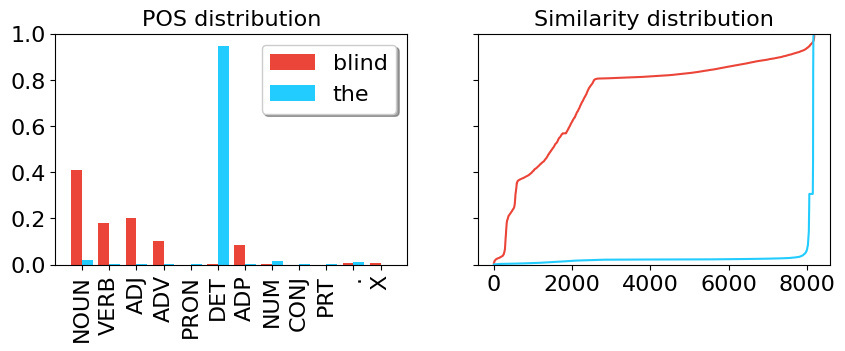
\includegraphics[width=0.8\linewidth]{chapters/syntatic-smoothing/figures/distributions.png}
    \caption{Part-of-speech distributions and similarity distributions for the subword tokens ``blind'' and ``the''. Similarities are computed as cosine-similarities against every other token in the vocabulary and sorted.}
    \label{fig:distributions}
    \vspace{-1em}
\end{figure}

\subsection{Smoothing the Backpropagation Signal}\label{section:smoothing}

Modern pre-training objectives implement likelihood maximization using a cross-entropy loss between the label of the correct word and predicted probabilities from a forward pass of the model. \texttt{Syntactic Smoothing} makes a small adjustment. Instead of a one-hot encoding, the target vector $t$ becomes a distribution across the entire vocabulary with some of the signal on the correct label $j$ and the rest of the signal distributed across all other tokens $i$ according to the syntactic similarity metric used:
\begin{equation}
\label{eq:signal-distribution}
    t_i=\left\{
  \begin{array}{@{}ll@{}}
    (1-\alpha), & \text{if}\ i=j \\
    \frac{s(i,j)}{\sum_{k=0}^{|V|}{s(i,k)}} \times \alpha & \text{otherwise}
  \end{array}\right.
\end{equation}

\noindent
where $\alpha$, the smoothing parameter, determines the proportion of the error signal reserved for the correct word and $s$ is our part-of-speech similarity metric. We experiment with different values for $\alpha$, noting that $\alpha=0$ is the standard likelihood maximization task. We also investigate the use of a pacing function that linearly decreases $\alpha$ so that at the start of training the majority of the signal is propagated to other syntactically similar tokens and by the end of training nearly all of the error signal is sent to the correct token to ensure that the model still optimizes perplexity. 

In practice, we also find it beneficial to apply a temperature scaling function to the syntactic similarity distribution. Thus, rather than using the raw syntactic similarity scores, $s(i,j)$, in \cref{eq:signal-distribution}, we use the temperature-scaled similarity scores:

$$
s'(i,j) = \frac{\exp\left(\frac{s(i,j)}{\tau}\right)}{\sum_{k=1}^{|V|} \exp\left(\frac{s(i,k)}{\tau}\right)}
$$
where $\tau$ defines the temperature which we set to $\tau=0.025$.

\subsection{Experimental Setup}
\label{subsection:experimental_setup}

Our experiments focus on smaller language models and datasets due to computational constraints and the particular challenges of generalizing to uncommon instances under resource-constrained training conditions \citep{warstadt2023babylm1,diehlmartinez2023climb}. 

\paragraph{Data} \label{paragraph:data} We use the dataset published as training data for the BabyLM challenge at the 2023 CoNLL workshop \citep{warstadt2023babylm1}. It contains roughly 10 million tokens sampled from pre-existing datasets, covering a wide range of domains including transcribed speech (both adult-directed and child-directed), movie subtitles, Wikipedia articles, and books. The dataset was constructed to be similar to the input received by children --- 56\% comes from transcribed speech and 40\% comes from sources intended for children.

\paragraph{Model} We use a small 8-layer encoder-style RoBERTa model with pre-layer normalization \cite{huebner2021babyberta}. We use the same hyper-parameters as the base model in \cite{diehlmartinez2023climb}. We use a BPE tokenizer \citep{sennrich2016bpe} with a vocabulary size of 8192 as recommended in previous work \cite{diehlmartinez2023climb}. 

\paragraph{Evaluation} We evaluate the BLiMP frequency bias of our models, as defined in \cref{section:freq-bias}, on the evaluation set of BLiMP. To compute anisotropy we use the formulation defined in \cref{eq:empirical-isotropy}; We sample 1,000 pairs of random word tokens with their surrounding context from the training set, and compute the cosine similarity of their hidden representation at each of the 8 layers of the RoBERTa model. To obtain a model's final anisotropy value, we average the anisotropy scores across the 8 layers. Additionally, we finetune and evaluate each model on two downstream sentence-level tasks, COLA \citep{warstadt2019cola} and SST-2 \citep{socher2013sst}, as well as two language inference tasks, MNLI \citep{williams2018mnli} and QNLI \citep{rajpurkar2016squad, wang2018glue}.


\paragraph{Baselines}

We introduce three types of baselines: 
\begin{enumerate}
    \item \textbf{Popular open-source transformer models}: OPT-125M \citep{zhang2022opt}, RoBERTa-base \citep{liu2019roberta}, and T5-base \citep{raffel2020t5}, pre-trained from scratch on the same dataset we describe in \cref{subsection:experimental_setup}. We use the default configuration for each model resulting in a varied number of parameters.
    \item \textbf{Base Model}: The small RoBERTa model described above without \texttt{Syntactic Smoothing}.
    \item \textbf{Label Smoothing}: The base model trained with label smoothing \citep{szegedy2016rethinking}.  We train a baseline with a low-level of smoothing ($\alpha=0.2$) and a mid-level of smoothing ($\alpha=0.5$). Note that \texttt{Syntactic Smoothing} can be seen as a linguistically-guided version of the standard label smoothing approach, in which the learning signal is distributed to all tokens uniformly.
\end{enumerate}


\paragraph{Our Models} We train our models with \texttt{Syntactic Smoothing} using the same two $\alpha$ values as the label smoothing baselines to facilitate comparison. We also run variants using the linear pacing function presented in \cref{section:smoothing} which linearly decreases the smoothing from an initial value of $\alpha$ to zero across training. For these variants, we use the same two values of smoothing, as well as an additional high value of $\alpha=0.8$ giving a total of five \texttt{Syntactic Smoothing} variants. We do not include unpaced \texttt{Syntactic Smoothing} with a high value of $\alpha$ as initial experiments found that distributing such a high proportion of the learning signal away from the correct token leads to high perplexity and poor downstream performance.

\section{Results}
\label{sec:results}

\begin{table*}[ht!]
    \centering
    \small
    \begin{tabular}{ll||cc|ccccc}
    \toprule
    \textbf{Model}  & $\alpha$ & \textbf{Bias}  & \textbf{Anisotropy} & \textbf{BLiMP} & \textbf{COLA} & \textbf{SST-2} & \textbf{MNLI} & \textbf{QNLI}  \\
    \midrule
    OPT   & - & 10.6 & - & 63.2 & 64.6 & 81.9 & 57.6 & 61.5\\
    RoBERTa & - & 13.7 & - & 69.8 & 70.8 & 87.0 & 73.2 & 77\\
    T5      & - & 6.2 & - & 58.3 & 61.2 & 78.1 & 48.0 &  62.0\\
    \midrule
    \midrule
    Base Model & -&9.8 & 51.3 & 71.4 & 71.4 & 82.9 & 69.6 & 79.7 \\
    \midrule
    \multirow{2}{*}{\makecell[l]{\texttt{Label}\\\texttt{Smoothing}}} &Low & 5.5 & 40.2 & 73.2 & 70.7 & 84.0 & \textbf{70.1} & 80.0 \\
    &Mid & 2.7  & 40.3 & 73.0 & 71.5 & 82.2 & 69.0 & 79.4 \\
    \midrule
    \multirow{5}{*}{\makecell{\texttt{Syntactic}\\\texttt{Smoothing}}}&Low  & 2.9 & 39.7 & \textbf{73.2} & 70.7 & 84.9 & 69.7 & 79.2 \\
    &Mid  & \textbf{-0.2} & 33.8 & 72.1 & \textbf{71.9} & 83.5 & 67.2 & 79.4 \\
    &P. Low & 7.4 & 39.9 & 71.9 & 70.5 & \textbf{85.2} & 70.0 & \textbf{80.4}\\ 
    &P. Mid& 5.7 & 34.5 & 72.3 & 71.8 & 84.0 & 68.2 & 78.9\\ 
    &P. High & 5.2 & \textbf{31.0} & 72.2 & 70.5 & 83.7 & 67.7 & 79.1 \\ 
    \bottomrule
    \end{tabular}
    \caption{\label{tbl:full-results} We report bias~($\downarrow$), anisotropy~($\downarrow$), BLiMP~($\uparrow$) score, and accuracy or correlation scores ($\uparrow$) on two downstream sentence-level tasks -- COLA and SST-2 -- and two downstream language inference tasks -- MNLI and QNLI -- for our MLM baseline, two label smoothing (LS) baselines, and five \texttt{Syntactic Smoothing} variants. Paced (P. Low, Mid, High) variants use linear pacing to reduce the smoothing factor to zero over training.}
\end{table*}

Our results are summarized in \cref{tbl:full-results}. We find that our method reduces frequency bias while retaining strong language modeling capabilities. At the same time, we observe that the models with the lowest frequency bias also demonstrate the lowest anisotropy. We then extend our analysis beyond the specific phenomenon of frequency bias and anisotropy by examining the impact of \texttt{Syntactic Smoothing} on the linguistic generalization capabilities of the model and its downstream performance after finetuning. Finally, we find that an alternative syntactic scoring metric leads to similar results as the cosine-based definition.

\begin{figure}[ht!]
    \centering
    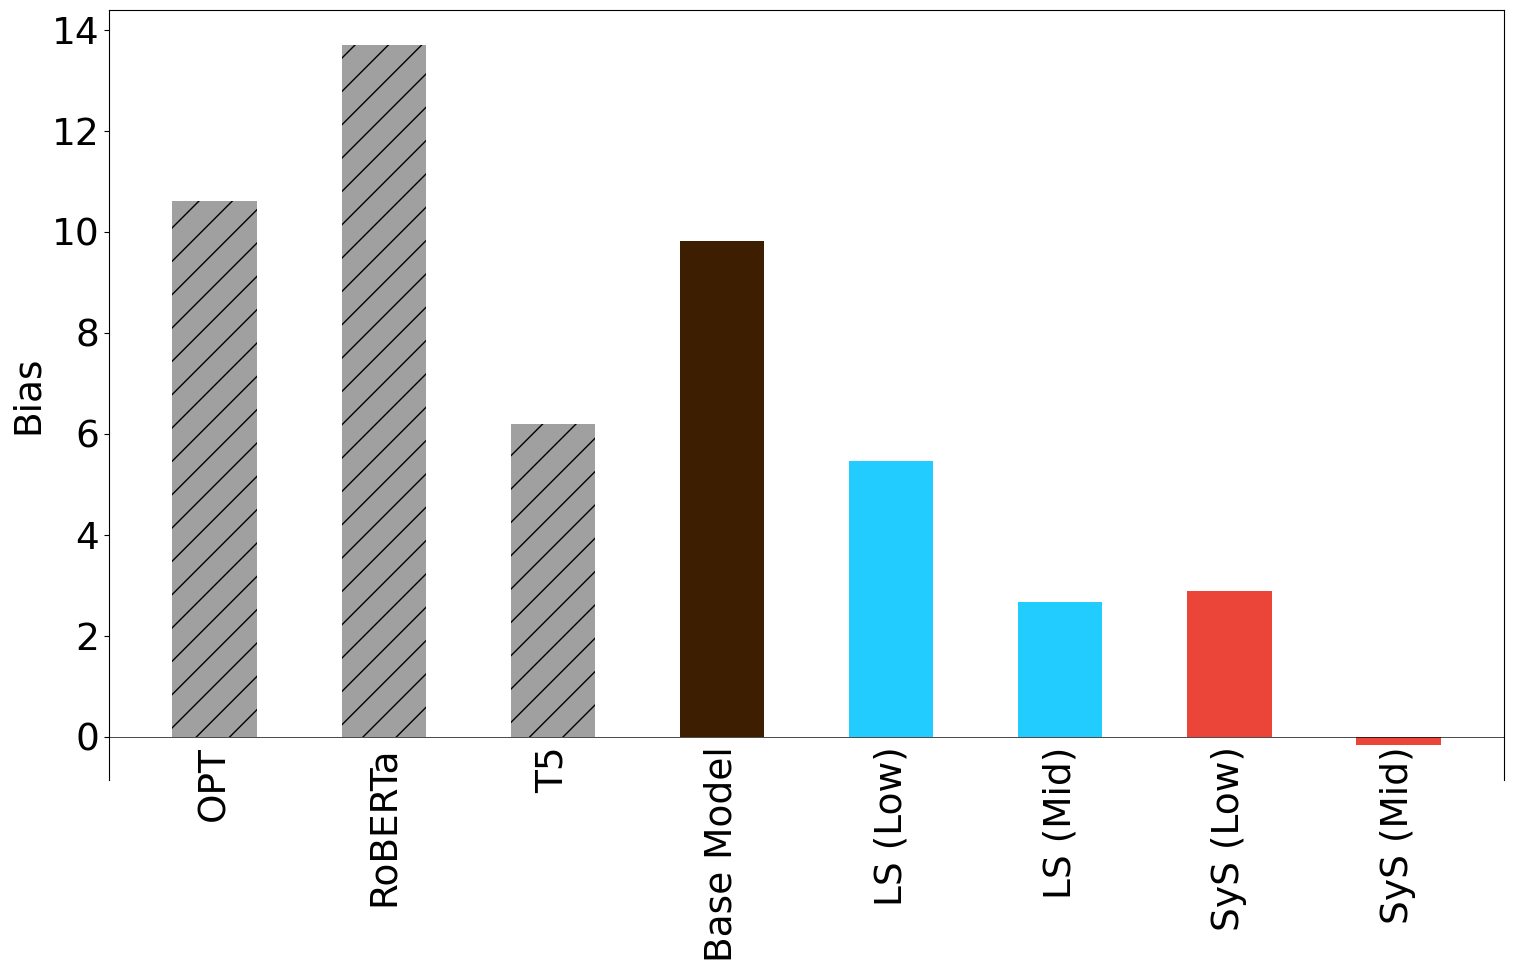
\includegraphics[width=0.7\linewidth]{chapters/syntatic-smoothing/figures/biases.png}
    \caption{Frequency bias plotted for the three open source pre-trained models, our base model, the two label smoothing (LS) baselines and our two \texttt{Syntactic Smoothing} (\texttt{SyS}) models.}
    \label{fig:biases}
    \vspace{-1em}
\end{figure}

\subsection{Anisotropy and Frequency Bias}
We conduct analyses to inspect the learning dynamics of our method and its effect on frequency bias and anisotropy in more detail. 

\paragraph{\texttt{Syntactic Smoothing} reduces frequency bias.}
We find that all four pre-trained models exhibit strong frequency bias (see \cref{fig:biases}); they are more likely to incorrectly prefer ungrammatical sentences if they contain tokens that occur more frequently during training. This confirms our hypothesis that the evaluation of generalization capabilities is obfuscated by frequency effects. 

By contrast, the two \texttt{Syntactic Smoothing} variants successfully reduce the frequency bias. The frequency bias is almost completely removed in the case of the \texttt{Mid} variant, which distributes exactly half of the training signal to syntactically similar tokens. We further observe that the Label Smoothing baselines also reduce bias but to a lesser extent than the corresponding \texttt{Syntactic Smoothing} models with the same degree of smoothing. 

\begin{figure}[ht!]
    \centering
    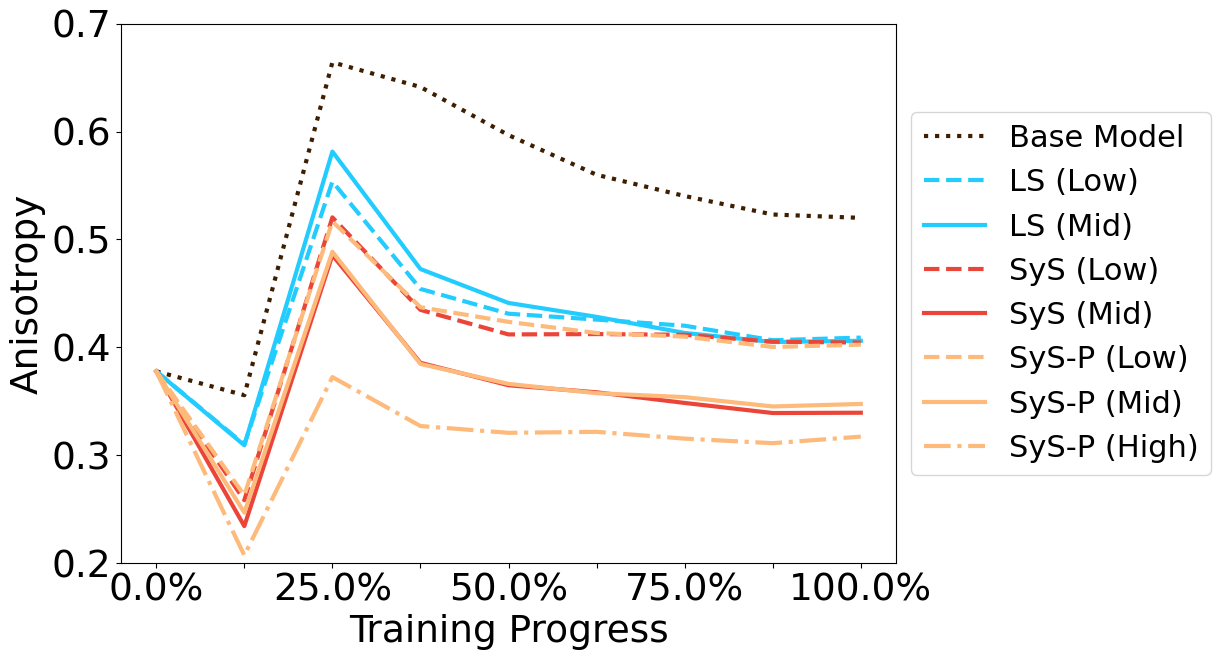
\includegraphics[width=0.7\linewidth]{chapters/syntatic-smoothing/figures/anisotropy-learning-dynamics.png}
    \caption{Anisotropy learning dynamics plotted for the baseline RoBERTa model, the two label smoothing (LS) baselines and our \texttt{Syntactic Smoothing} (\texttt{SyS}) models. Values in parentheses indicate the degree of smoothing.}
    \label{fig:anisotropy-learing-dynamics}
    \vspace{-1em}
\end{figure}

\paragraph{\texttt{Syntactic Smoothing} reduces anisotropy.}

As shown in \cref{tbl:full-results}, \texttt{Syntactic Smoothing} reduces anisotropy over both the base model and label smoothing baselines.\footnote{Note that we do not compute the anisotropy for the three open-source pre-trained models (OPT, RoBERTa, T5) because these models use different architectural configurations than the models we train (e.g., larger hidden dimensions).} Label smoothing reduces anisotropy, but not to the same extent as our \texttt{Syntactic Smoothing} models. To better understand how anisotropy develops in a model, we compute the model's anisotropy scores at eight checkpoints during training, as shown in \cref{fig:anisotropy-learing-dynamics}. We find that a greater degree of smoothing leads to a greater reduction in anisotropy for our \texttt{Syntactic Smoothing} variants (it is less clear if this is the case for label smoothing), supporting our hypothesis that syntactic initialization helps promote better representation learning across the model's vocabulary. We also find that the pacing method leads to lower anisotropy than the flat method, with \texttt{SyS}-P (High) achieving the lowest anisotropy throughout.

Over the course of training, we observe a consistent double-dip trend: an initial dip followed by a sudden rise, followed by a second slow decrease in anisotropy. The \texttt{Syntactic Smoothing} models do not see as large a sudden rise, maintaining a lower anisotropy throughout. To examine the learning dynamics in more detail, we also plot the evolution of the anisotropy across several layers of our baseline model and the \texttt{SyS}-P (High) variant, given in \cref{fig:anisotropy-layers}. Two observations stand out. The anisotropy of all layers in the \texttt{Syntactic Smoothing} model is lower than in the corresponding layers in the baseline model across the entire learning process. In both the baseline model and the \texttt{Syntactic Smoothing} model, earlier layers have lower anisotropy; this finding agrees with the same observation made by \citeauthor{ethayarajh2019contextual}. Notably, in the final layer—commonly used for sentence representations in downstream tasks—the anisotropy of the \texttt{Syntactic Smoothing} model remains consistently low and does not increase significantly during training, in contrast to the drastic fluctuation observed in the baseline model. 

\begin{figure}[ht!]
    \centering
    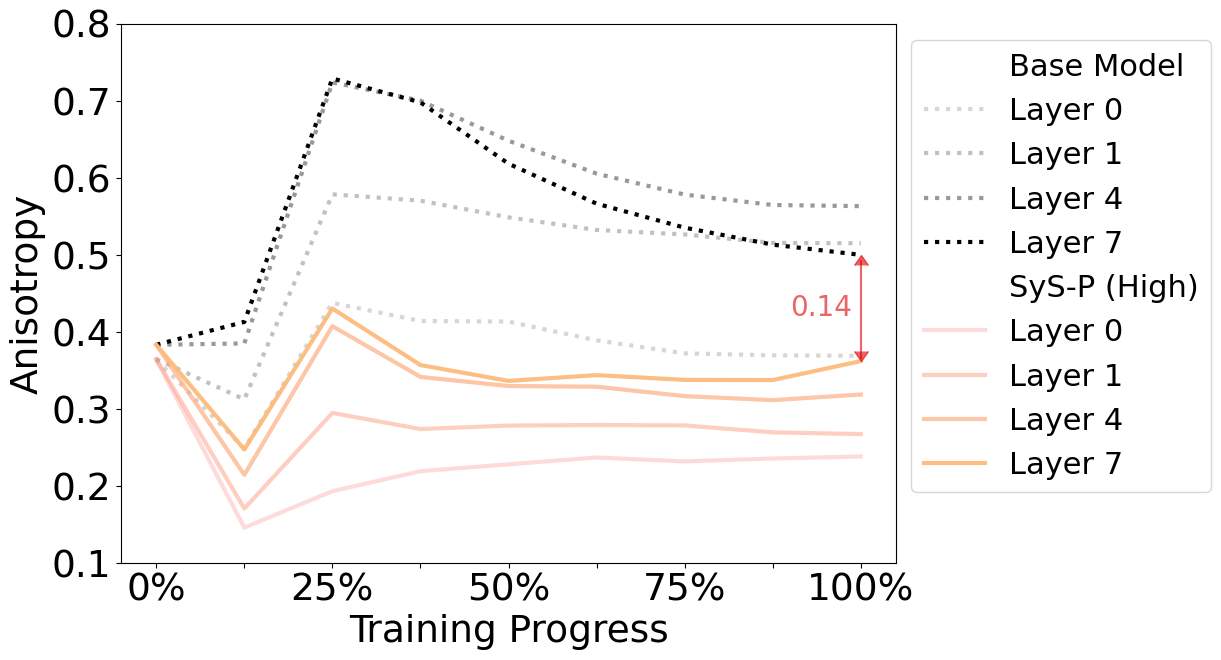
\includegraphics[width=0.75\linewidth]{chapters/syntatic-smoothing/figures/anisotropy-layers.png}
    \caption{Anisotropy learning dynamics plotted for the baseline model and the paced \texttt{Syntactic Smoothing} model with high smoothing, across some of the models' layers. We highlight the difference in anisotropy of the final layer across the two models at the end of training.}
    \label{fig:anisotropy-layers}
    \vspace{-1em}
\end{figure}

\paragraph{Frequency bias and anisotropy are correlated.}

For each model, we compute the model's frequency bias and anisotropy at multiple training stages. We plot the learning dynamics of anisotropy and frequency bias in \cref{fig:bias-anisotropy-correlation}, only including the points after 50\% of training has been completed to avoid the noisy first dip observed in the anisotropy dynamics above. We find a positive Pearson correlation of 0.73 and a polynomial goodness-of-fit $R^2$ score of 0.63 between these two metrics.

It is also evident that the pacing approach re-introduces frequency bias towards the end of training, as the degree of smoothing is linearly reduced to zero. It is noteworthy that the final anisotropy and bias are lower than the baseline model, and completing training without any smoothing may be beneficial for downstream tasks, as explored in the next section.

\paragraph{Frequency Bias Disproportionately Affects Content Words}
\label{section:word-class-versus-word-frequency}

\begin{figure}[ht!]
    \centering
    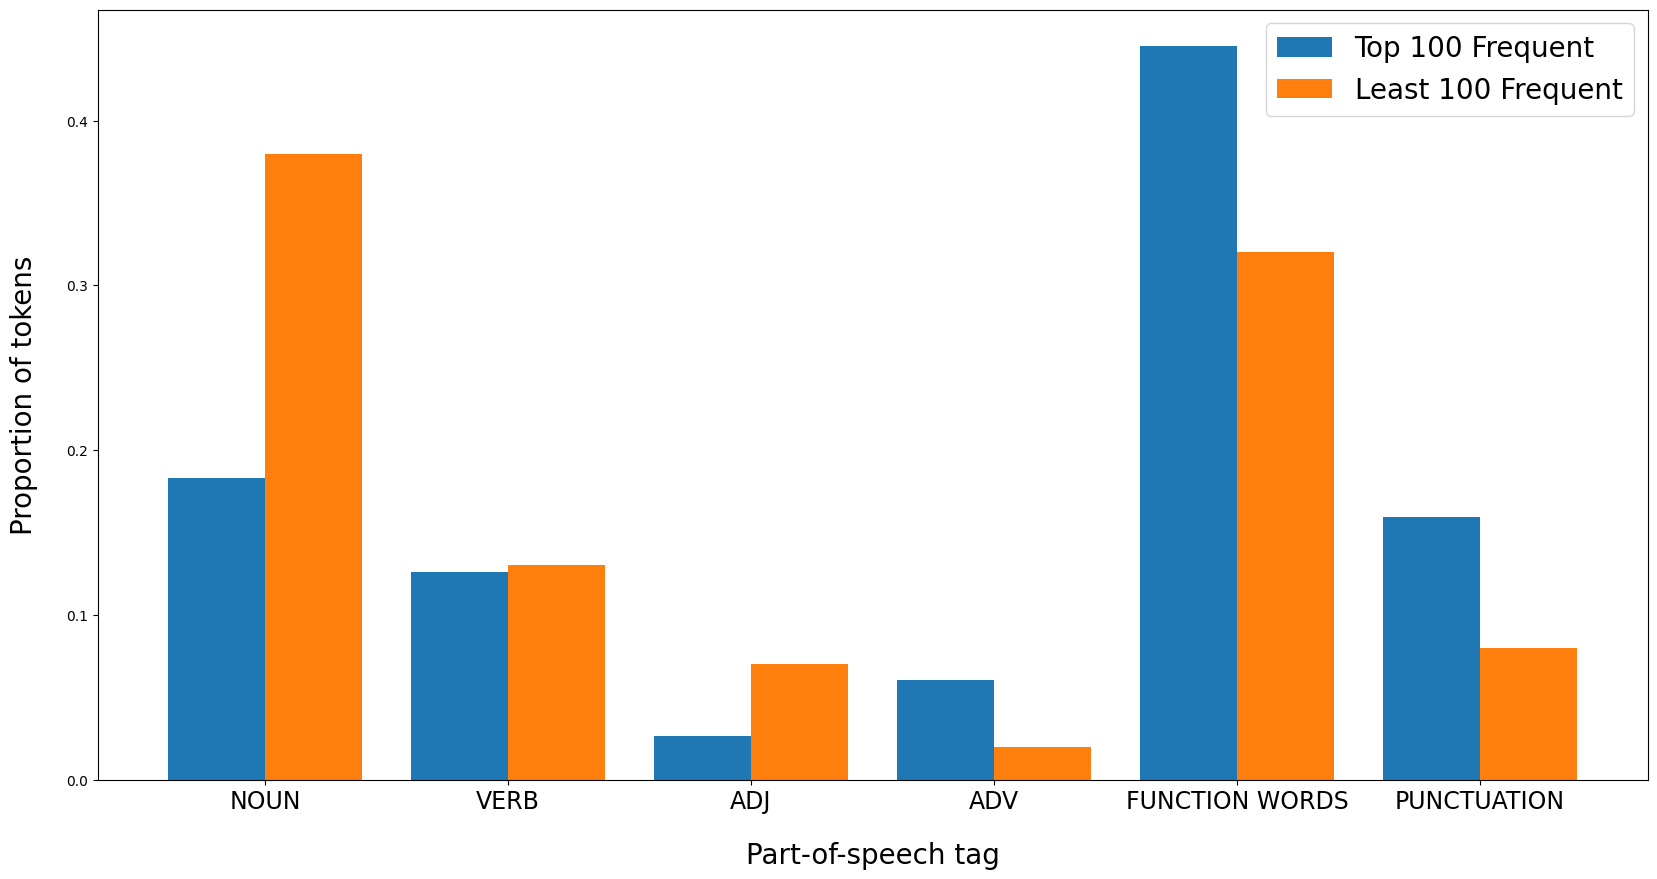
\includegraphics[width=0.65\linewidth]{chapters/syntatic-smoothing/figures/top_versus_bottom_pos_dist.png}
    \caption{Distribution across POS tags of the top versus bottom 100 most frequent tokens.}
    \label{fig:top-100-pos-dist}
\end{figure}

To better understand the linguistic categories most impacted by frequency bias, we analyze the relationship between token frequency and syntactic class. Specifically, we compare the POS tag distributions of the top 100 most frequent tokens and the bottom 100 least frequent tokens in our training data. 

We find that content words—especially nouns—are over-represented in the low-frequency tail of the distribution, while function words dominate the high-frequency tokens. \cref{fig:top-100-pos-dist} illustrates this disparity. This suggests that frequency bias in language models may disproportionately hinder the learning of specialized vocabulary, particularly rare nouns and content-bearing expressions. It also reinforces the importance of a smoothing strategy that supports lexical generalization by leveraging syntactic structure.


\begin{figure}[ht!]
    \centering
    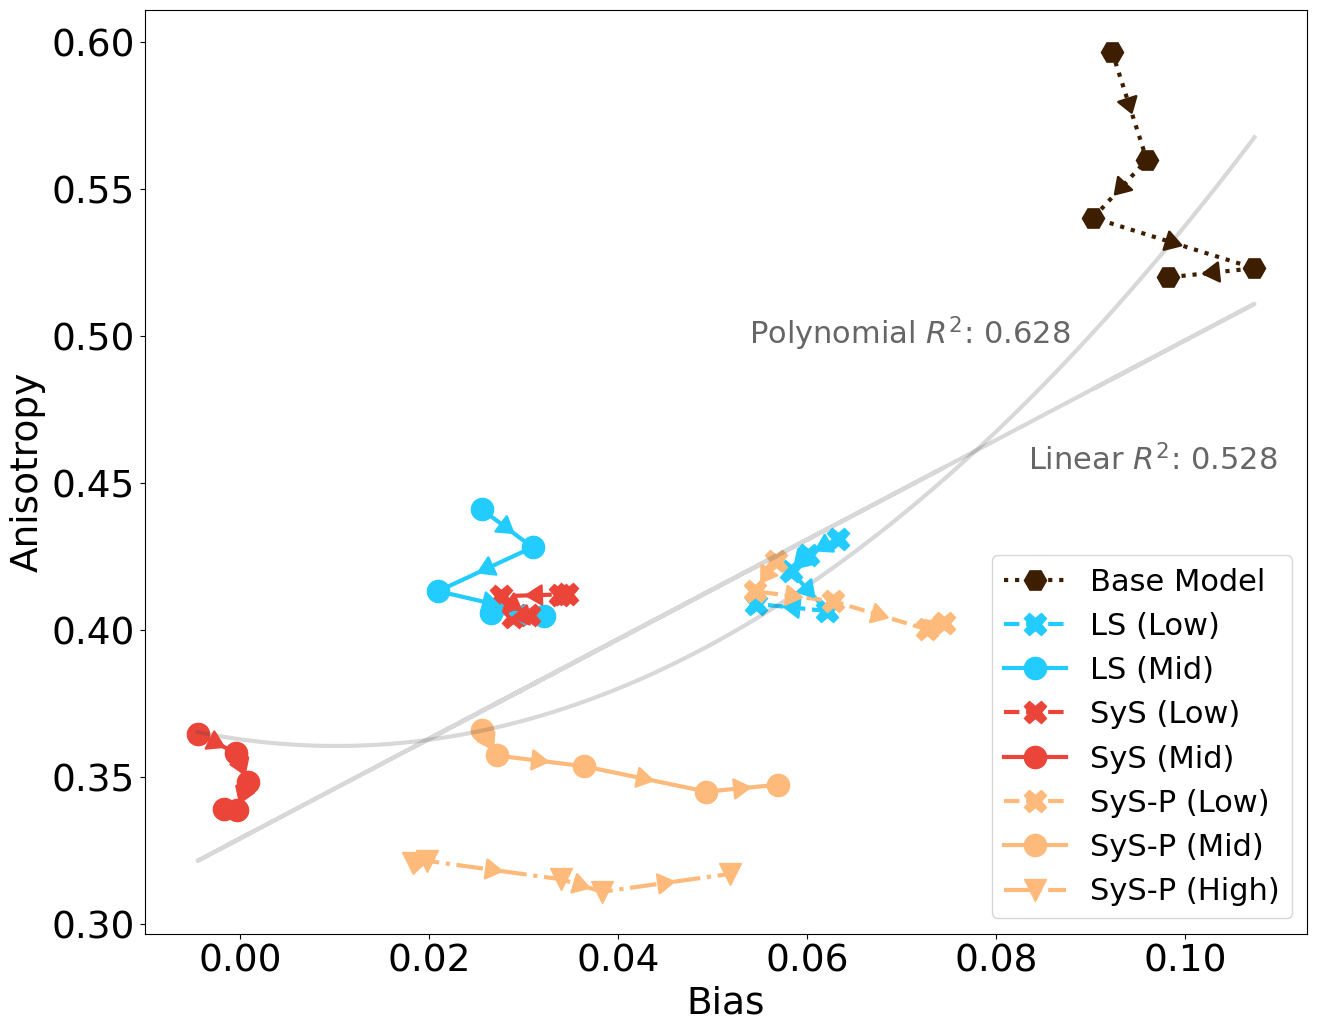
\includegraphics[width=0.75\linewidth]{chapters/syntatic-smoothing/figures/bias-vs-anisotropy.png}
    \caption{Pairs of anisotropy, and frequency bias for the baseline RoBERTa model, the two label smoothing baselines and our \texttt{Syntactic Smoothing} models. The arrows indicate increasing training progress (starting after 50\% of training has completed).}
    \label{fig:bias-anisotropy-correlation}
\end{figure}

\subsection{Effects of Smoothing on Downstream Tasks}
While our method primarily aims to enhance the representation of infrequent tokens, we sought to investigate the potential for improvement in standard evaluation measures, given the limited number of affected test instances. Nonetheless, we observe that all the \texttt{Syntactic Smoothing} models, as well as the label smoothing models, achieve better BLIMP scores than our baseline model (see \cref{tbl:full-results}). These results suggest that methods that smooth label distributions, whether through a syntactic prior or a simpler uniform smoothing approach, enhance the representation of all tokens, including the more frequent ones.

We had concerns that softening the frequency bias with our method might lead to degraded performance in downstream tasks for which frequency can be a strong proxy. As a control condition, we finetune our model on two sentence-level tasks (COLA, SST-2) and two language inference tasks (MNLI and QNLI), both of which are part of the GLUE \citep{wang2018glue} benchmark. We find that none of the \texttt{Syntactic Smoothing} objectives result in substantial performance degradation on these NLU tasks (see the last four columns of Table~\cref{tbl:full-results}), and in fact note that for some tasks, such as SST-2, the \texttt{Syntactic Smoothing} models yield uniform increases in performance. While not comparable apples-to-apples, we report NLU performance for the open-source baselines in \cref{tbl:full-results} as a point of reference. 

\subsection{Alternative Measures of Syntactic Similarity}

In \cref{sec:sim} we define the syntactic similarity score that is used by the \texttt{Syntactic Smoothing} approach as the cosine similarity between POS distributions. To examine how this specific choice of similarity metric impacts our approach, we replace the cosine-based definition with a Jensen Shannon-based definition:
$$ \frac{1}{2}\big[ \text{KL}(M_i, M_j ) + \text{KL}(M_j, M_i)\big],$$
where KL$(M_i, M_j)$ is the Kullback-Leibler divergence between the POS distributions, $M_i$ and $M_j$, for the vocabulary items $V_i$ and $V_j$.

\begin{table}[ht!]
\centering
\small
\begin{tabular}{l||cc|ccccc}
\toprule
\textbf{Model}  &  \textbf{Bias}  & \textbf{Anisotropy} & \textbf{BLiMP} \\
\midrule
Base Model & 9.8 & 51.3 & 71.4  \\
\midrule
\texttt{SyS} (Mid) \hspace{0.42cm} [JS]  & 3.6 & 34.7 & 71.3 \\
\texttt{SyS} (Low) \hspace{0.38cm} [JS]  & 4.1 & 34.6 & 73.3  \\
\texttt{SyS}-P (High) \hspace{0.05cm} [JS] & 6.6 & 36.7  & 72.5  \\ 
\texttt{SyS}-P (Mid) \hspace{0.15cm} [JS] & 8.4 & 39.1 &  73.0 \\ 
\texttt{SyS}-P (Low) \hspace{0.12cm} [JS] & 5.0 &  34.5 & 72.9 \\ 
\bottomrule
\end{tabular}
\caption{\label{tbl:jsd-similarity-metric-results}
Results for bias~($\downarrow$), anisotropy~($\downarrow$), and BLiMP~($\uparrow$) score for \texttt{Syntactic Smoothing} (\texttt{SyS}) models that use a Jensen Shannon-based [JS] definition of the similarity metric.}
\end{table}

Summarized in \cref{tbl:jsd-similarity-metric-results}, we note that the effect of using a Jensen Shannon-based definition of the similarity metric yields a similar (albeit slightly smaller) decrease in frequency bias and anisotropy, as compared to the standard cosine-based definition of the similarity metric.   

\section{Conclusion}
\label{sec:conclusion}

This chapter has addressed a core limitation of current language models: their difficulty in generalizing to rare or novel words due to an overreliance on frequency statistics. While human learners can infer grammatical roles and meanings from structural context, a process often referred to as syntactic bootstrapping, most language models lack this inductive bias. As a result, they tend to prioritize high-frequency tokens, leading to frequency bias and degraded representations of infrequent words.

We proposed \texttt{Syntactic Smoothing}, a cognitively motivated training method that distributes the learning signal for each token across other syntactically similar tokens. Using part-of-speech distributions as a simple approximation for syntactic similarity, this approach allows low-frequency tokens to benefit from the learning dynamics of more frequently observed counterparts. In doing so, it operationalizes the human strategy of learning by structural association.

To evaluate this method, we introduced a new diagnostic for frequency bias, measuring the degree to which a model incorrectly prefers ungrammatical but frequent alternatives. We found that \texttt{Syntactic Smoothing} significantly reduces this bias and also decreases anisotropy in the representational space. These gains were achieved without sacrificing downstream task performance, suggesting that structural cues can support lexical generalization even in small-scale or low-resource training settings.

By connecting insights from cognitive science with concrete modifications to training, this chapter moves beyond architectural changes and explores how the learning process itself can be made more human-like. If curriculum learning structures what is learned and when, \texttt{Syntactic Smoothing} focuses on how internal representations evolve to support abstraction and generalization.

In the next few chapters, we take a closer look at this process. How do language models internalize linguistic structure over time? What patterns of learning emerge during training, and how do they compare to those observed in human learners? Building on the methods introduced here, we now turn to analyzing the dynamics of learning within neural language models.
